%% We use `subfiles' package
\documentclass[preamble.tex]{subfiles}
\begin{document}

\clearpage

\chapter{Background}

\section{Runtime Fusion Systems}

\subsection{DESOLA - Delayed Evaluation Self Optimising Linear Algebra}

Delayed Evaluation Self Optimising Linear Algebra (DESOLA) \cite{RMKB06} is a C++ active library which was designed to explore the benefits of runtime code generation and optimisation for scientific computing. In contrast to DPH, DESOLA puts portability across compilers as one of its priorities, thus it may provide several insights in doing thing differently. In particular, most of the interesting code generation and optimisation happens at runtime. Quoting the authors of the library, they take the following approach:

\begin{description}
\item [{Delay~library~call~execution}] Calls made to the library are used to build a “recipe” for the delayed computation. When execution is finally forced by the need for a result, the recipe will often represent a complex composition of primitive calls.
\item [{Generate~optimised~code~at~runtime}] Code is generated at runtime to perform the operations present in the delayed recipe. In order to improve performance over a conventional library, it is important that the generated code should execute faster than a statically generated counterpart in a conventional library. To achieve this, we apply optimisations that exploit the structure, semantics and context of each library call. Compiled recipes are cached to limit overheads, but need to be executed enough times to offset the cost of the initial compilation.
\end{description}

\begin{figure}
\begin{centering}
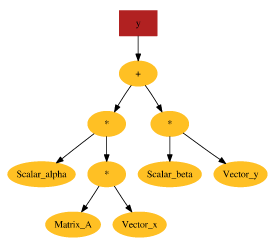
\includegraphics{img/DESOLA-running-example}
\par\end{centering}

\caption{\label{fig:Lib:DESOLA-DAG}{An example DAG. The rectangular node denotes a handle held by the library client. The expression represents the matrix-vector multiply function $y = \alpha Ax + \beta y$.}}
\end{figure}


Figure \ref{fig:Lib:DESOLA-DAG} shows a tree, or more generally a directed acyclic graph (DAG), accumulated during the evaluation of a matrix-vector multiply function. The important thing to note is that the authors insist on that DAG is a more effective way to record computations than a tree as it exposes the sharing of {}``recipes'' among handles in the client code. This may not always be possible in a purely functional context and will have to be explored. The actual fusion algorithms employed in DESOLA are not explained in much detail. The authors found that their achievements in fusion using the information only available at runtime compensated the runtime code generation cost for many real sized problems. The authors also believe that the benefits of array contraction will be more noticeable once they add support for sparse matrices and similar irregular data structures to their library. As this is the focus of DPH, array contraction may be beneficial to look at in more detail.

Overall, the approach of delaying the evaluation until it it required seems promising and aligns well with Haskell's approach to lazy evaluation (only from the ideological point of view, since the performance is the first priority for DPH).



\section{Stream Processing and Data Flow Languages}

\section{Darte}

Done in Fortran. While more lowlever, the first thing it does is to do dep analysis and separate into several loop. All the fusion is done after that. In this way we actually start one level below. We already have independet loops with most combinators introducing at least one loop into the graph.

\section{On clustering}

Most clustering problems are expressed in compile time and in general take NP to complete. For a medium sized DPH program you have (N) combinators at a time. This shoots the problem outside reasonable compilation times. With a good set of ILP heuristics and without looking for a perfect solution a performat ILP solver can bring this down to reasonable amount of time. It is worth noting two things: at compile time you can indeed see the complete graph at once which is unlikely at runtime. Certain things will be forced and reduced to manifest arrays before time (give an example). Thus there may not be such a high number of things to solve. Also, any time a simple linear pipeline of combinators is encountered and their rate and access pattern (i.e. type) are the same, they can all be reduced to one combinator for the purposes of clustering. This way, it may well be possible that the graphs to analyse for clustering may become very small.

Two other techniques which may drammatically reduce the graph to be analysed is simple runtime forcasting:
- At compile time you may not always see the sizes of arrays to be computed. You have to assume you will need to fuse everything to our best abilities. However, as the author found in his work on Parallelisation avoidance, only a handful of combinators in an average DPH program are actually majour contributors to the runtime. As such, we may often be able to skip clustering and subsequent compilation altogether. Performing a cheap array computation may just suffice. Working with the resulting manifest arrays for fusion where it is truely beneficial is much easier than with a set of combinators which only introduce ``noise'' into the actual runtime of the program.

\section{Summary}

This section has reviewed some of the array fusion frameworks covering
a number of:
\begin{itemize}
\item languages (C++, Haskell),
\item applications (algebraic libraries, general purpose list library, data parallel framework),
\item approaches (runtime evaluation graph optimisation, equational fusion based on rewrite rules).
\end{itemize}
The discussion in the next section will be based on the fusion frameworks described above.


\clearpage
\chapter{LiveFusion - A Runtime Fusion System}

The current project was motivated by Data Parallel Haskell project. Even though much of the design of the new fusion system is decoupled from any particualar system targetting it, the fusion frameworks designed specifically for Haskell were the first to turn to. The Background section discussed three of them: Shortcut Fusion, Stream Fusion and Functional Array Fusion. Glasgow Haskell Compiler's rewrite rules functionality plays crucial rule in all three of them. This is not coincidental:
\begin{itemize}
\item Compile-time term rewriting is fundamental optimisation technique in the implementation of functional programming languages \cite{Pey87}. Exposing it to the user \cite{PTH01} makes it an attractive way to expose compiler functionality to pure library code
\item Inlining \cite{PM02} is another technique which is crucial in compilers like GHC which heuristically removes superfluous levels of indirection in the original code. As a side effect it provides more opportunities for term rewriting to happen
\item Haskell is a purely functional language therefore valid term rewriting can be done without a sophisticated analysis of side effects. Rewriting would generally be unsafe in a non pure context
\item (In the case with Stream Fusion) it is reasonable to rely on the existence of certain compiler optimisations since DPH relies on GHC and is not designed for other Haskell implementations
\end{itemize}
The above statements suggest that compile time equational fusion seems like a natural choice for the Haskell programming language. This is especially valid for Stream Fusion where the authors were able to achieve, through inlining, rewriting and compiler optimisations, the speed of handwritten code. Moreover, the generated code for many examples was the same as a human programmer would normally write if top performance was required. However, the strong dependence on the optimisation systems of such a complex system as GHC makes the fusion frameworks fragile and non-portable.

One of the cases in which equational fusion breaks is when two array operation do not end up being adjacent after inlining. This may happen due to the so called \emph{let floating} optimisation in GHC \cite{PPS96}.

%% TODO find a breaking example in DPH and list it here This optimisation is designed to avoid duplicating work. When GHC finds two identical terms in an expression and considers them large enough to benefit from computing them only once, it \emph{floats} them out to a new \emph{let} binding outside of the expression. This optimisation is the opposite of inlining. If the term that was forcibly floated out would have otherwise completed a pattern for a fusion rule, that fusion opportunity is missed.

The other problem with equational fusion is that \emph{sharing} is not clearly defined. This is related to the above problem. Sharing prevents large amounts of work from being duplicated. Aggressive unconditional inlining would have introduced a major inefficiency for programs in which the result of a pipeline of costly array operations is independently used in more than one place. Recomputing the shared portion may result in a noticeable performance hit.

Both of the above two problems suggest that correct inlining plays a major part in the process of fusion. It also suggests that the decisions taken by the inliner do not always result in the optimal code for exploiting fusion. 

One of the goals of the current work is to reduce the dependency of successfully exploited fusion opportunities on the behaviour of the inliner. It was decided to explore the possibility of performing fusion at runtime of the program. That would eliminate the need for the inliner at least for the part of decision making when fusing array operations together. The DESOLA library, while designed for C++, serves as a starting point for performing fusion at runtime. The new framework would reuse its approach of constructing a dependence tree. When an array computation is later forced by a catamorphism, the tree can be optimised yielding an equivalent computation in a fused form.

The very first design decision to make would be the way to represent delayed array operations as nodes in the tree. Haskell's ability to delaying function application and effortless function composition to create new functions has lead the author to reusing the approach of Functional Array Fusion. In our case each node in the tree either represents a delayed array computation or holds a precomputed array in memory. The tree represented in this manner may be optimised and evaluated at any time to produce a manifest array in memory. All of the library's interface functions can then be implemented in terms of nodes in the tree.

%%As a special case, the catamorphic functions, not only obtain a new
%%delayed array handle but also force the evaluation of the tree.

%%The next feature of the new framework to be implemented would be the
%%support for segmented array operations. Segmented array operations
%%are central to DPH. Implementing them would complete the interface
%%of the library. Luckily the authors of Functional Array Fusion have
%%provided one solution for it. Implementing it would require modifying
%%the the type signature of the mutator function and generalising the
%%\emph{loop} combinator to support segment boundaries.

(TODO decide what to do with the following paragraphs, it should probably go in background section) At a minimum give overview of:
\begin{itemize}
\item Sharing recovery
\item New loop representation
\item Code gen for new loop representation
\item Code compilation and loading
\item Finish by saying that these will be discussed in turn in the coming sections
\end{itemize}

The next major feature required for DPH to be used with the new backend as intended would require adding support for distributing computations over the available processing elements. At present time DPH has two backends: one purely sequential and one parallel. However, they are not entirely independent. The parallel backend is concerned with only the following:
\begin{itemize}
\item splitting (chunking) arrays and distributing them among a \emph{gang of threads}
\item calling a sequential implementation from the sequential backend on each chunk
\item joining the chunks from the finished parallel operations
\item statically removing as many synchronisation points as possible (split-joins) 
\end{itemize}

The last item on the list was parallel backend's own fusion system described \vpageref{Lit:DPH-fusion-levels}. Fusion in the sequential backend occurs only after that in the parallel backend (more precisely after a split and before the next join). On one hand that allows the two fusion systems to be independent. However, considering the nature of the new sequential backend it may sometimes do no work between the two split-joins. Indeed, we said initially that we were only forcing the evaluation of the tree when reaching a catamorphism. A dynamic technique for eliminating superfluous synchronisation points in the context of functional programming languages has been suggested in {[}Operator fusion{]} under the name Operator Fusion for the Scala programming language. It is a simple algorithm with requires every function in the library to be classified according to:
\begin{itemize}
\item whether or not the inputs are consumed sequentially (\emph{map} vs. \emph{backpermute}),
\item whether or not the outputs are produced sequentially (\emph{map} vs. \emph{permute}),
\item whether or not load unbalancing may happen (\emph{map} vs. \emph{filter})
\end{itemize}

While the \emph{loop} operator presumes traversing the array from left to right, the aforementioned work may prove to be useful when adjusting the parallel backend.

Lastly, there are two optional features that may be researched and possibly implemented:
\begin{enumerate}
\item Traversing more than one array one after the other, e.g. using \emph{concat} or \emph{concatMap}
\item Sharing recovery and fusion preserving sharing. Normally, it is not possible in the purely functional context to refer to the same tree node from two other nodes to share computation between them. However turning the tree into a Directed Acyclic Graph (DAG) to enable sharing was found to be detrimental for performance and one of the performance bottlenecks in DPH (TODO ref latest paper). This problem has been researched in the context of Accelerate Domain Specific Language embedded in Haskell \cite{CKL+11} (TODO As well as a million other libs, sharing recovery is one of the two biggest problems in EDSL world). Fusion preserving sharing is a step up from sharing recovery enabling to continue running multiple computations in a fused manner (as opposed to first precomputing the shared portion of the DAG). This is unfortunately where Stream Fusion and other equational fusion frameworks fail. (TODO explain better)
\end{enumerate}


\IfNotCompilingAll{\bibliography{bib}}

\end{document}